%*******************************************************************************
%*********************************** First Chapter *****************************
%*******************************************************************************

\chapter{Posture Generation, state of the Art, Introduction}


\nomenclature[z-PG]{PG}{Posture Generation}
\nomenclature[z-IK]{IK}{Inverse Kinematics}
\nomenclature[z-DoF]{DoF}{degrees of freedom}
\nomenclature[x-I]{$\mathbb{I}_n$}{Matrix identity of dimension $n$}
\nomenclature[x-w]{$\wedge$}{cross product}
\nomenclature[z-mbg]{mbg}{Multibody Graph}
\nomenclature[a-F]{F}{a frame}
\nomenclature[a-W]{W}{the world frame}
\nomenclature[a-w]{w}{a wrench}
\nomenclature[a-f]{f}{a force}
\nomenclature[a-m]{m}{a moment}


\graphicspath{{Chapter1/Figs/Vector/}{Chapter1/Figs/}}

\section{List of contributions}
\begin{itemize}
  \item Generalities, introduction
  \item Presentation of the existing methods
  \item From Inverse Kinematics to Generalized IK/posture Generation/pose estimation (addition of articular limits, forces, stability etc.
  \item Topology of the parametrization space (Free-flyer, q, f, other)
  \item Formulation as a non-linear constrained optimization problem
  \item Adrien \& Karim's formulations
  \item Formulation of several types of cost/constraints
  \begin{itemize}
    \item Contact with plane surface
    \item Collision avoidance
    \item Auto-Collision avoidance
    \item Static equilibrium: Newton/CoM projection
    \item Forces in friction cones
    \item Articular limits
    \item Torque limits
    \item Torque minimization
    \item Goal Posture
  \end{itemize}
  \item Reasons why it is not enough and why we needed a new PG
    \begin{itemize}
      \item Having an easier way to formulate problems
      \item Avoid having to de some gymnastic to remain on manifolds
      \item Automatic variable management
      \item Robustness
    \end{itemize}
  \item Utilization of posture generation in planning
\end{itemize}


%%%%%%%%%%%%%%%%%%%%%%%%%%
%  SECTION INTRODUCTION  %
%%%%%%%%%%%%%%%%%%%%%%%%%%

\section{Introduction}
\label{sec:introduction}

The ultimate goal of robotics is to make robots realize some tasks.
The tasks, as well as the robot used to fulfill them are various.
For example, it can be a robotic arm building a car in a factory, a surgeon robot operating on a human, a submarine robot exploring the wreckages of a ship, a humanoid robot exploring and fixing a destroyed nuclear plant.

\begin{figure}[ht]
  \centering
  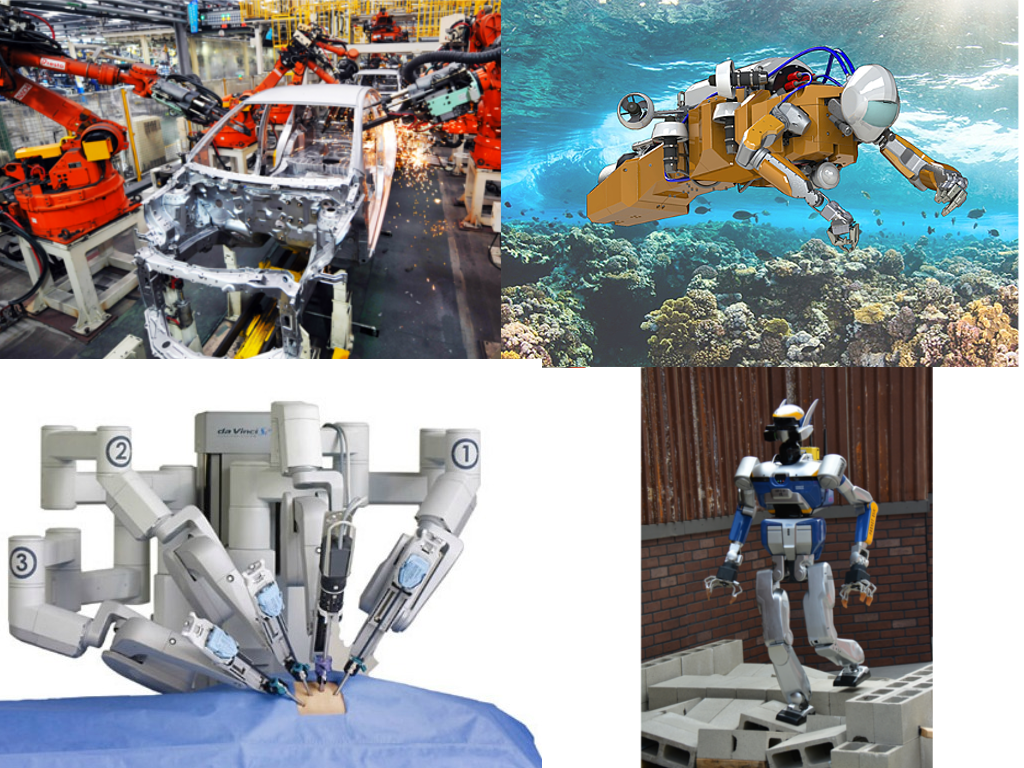
\includegraphics[width=0.9\textwidth]{various-tasks.png}
  \caption{Various robots doing various tasks}
  \label{fig:various}
\end{figure}

The DARPA Robotics Challenge has brought some light on the humanoid robots.
This competition brought together a large scope of robotics groups from universities, laboratories and private companies around a common goal: Make a robot succeed in several challenges without any human physical intervention.
The robots were expected to drive a car, open a door, climb stairs, cross debris, drill a hole in a wall, etc.
All those tasks can usually be broken down into sets of elementary tasks in human language.
Some typical examples of tasks for a robot can be "Put hand in contact with target", "Put foot on next step", "Avoid collision with that object", "Maintain stability" or "Look in that direction".
As is, those tasks do not mean anything for the robot.
A robot is made of a collection of bodies that are linked together by joints actuated by motors.
A robots configuration consists of the position and orientation of its base body, and the configuration of each of its joints.
Satisfying a task requires that the joints of the robot reach a configuration for which the task is satisfied.
The action of satisfying a task comes down to moving from an initial configuration to a goal configuration, figuring out the trajectory to follow and actually following it are the jobs of the trajectory generation and the control of the robot.
Those are by themselves some complete fields of robotics, and they have one thing in common, they both need to be given an initial configuration, a final configuration and sometime some intermediate configurations.
Finding those configurations is the job of what we call the Posture Generation (PG), which is the main topic of this dissertation.
There are two types of robots. The fixed-base robots and the mobile robots.
The first type of robots have fixed basis, the area that they can reach is predefined by their geometry and they are usually fully-actuated.
Which means that the robot has as many degrees of freedom(DoF) as actuators, Thus, for any joint configuration, a unique robots position is achieved.
On the contrary, mobile robots are under actuated, which means that the robot has more DoF than actuators.
Each link of the robot is actuated, but the position of the basis of the robot is the result of the configuration of the joints and of the contacts that the robot makes with the environment.
A mobile robot's position depends on the location of its contacts with the environment.
For biped robots evolving on a flat surface, a footstep planner can be used to decide of the sequence of steps to take so the robot can walk to its goal.

Humanoid robots are expected to move and achieve tasks in ways similar to humans.

On flat surfaces, they can walk based on a cyclic motion and the locations of footsteps can be generated by a footstep planner using some simplified models to maintain the robots stability.
In cumbersome and unstructured environments, we humans move in a non-gaited acyclic way: we choose appropriate parts of our body to create contacts with the surrounding environment in order to support the motion of the remaining parts while avoiding obstacles.
A whole motion is a sequence of contact creations and releases.

Since we are biped, we mostly use our feet to move.
As the environment becomes more difficult to cross, hands may come into play together with feet to help with the motion.
Narrow passages may even require other parts of our body (knees, elbows, back...) to make contact in order to support the motion.

In the past few years, our team has dedicated considerable efforts in proposing a general multi-contact motion planner to solve such cases of non-gaited acyclic planning.
Given a humanoid robot, an environment, a start and a final desired postures, the planner generates a sequence of contact stances allowing any part of the humanoid to make contact with any part of the environment to achieve motion towards the goal.
The planner's role is to grow a tree of contact stances iteratively, from a given posture, it tries to removes one of its contacts or to add a new one.
The tree grows, following some heuristics until the solution is reached.
A typical experiment with a HRP-2 robot achieving such an acyclic motion is presented in~\cite{escande:iser:2008}, and the planner is thoroughly described in~\cite{escande:ras:2013}.
Extensions of this multi-contact planner to multi-agent robots and objects gathering locomotion and manipulation are presented in~\cite{bouyarmane:ar:2012}, and preliminary validations with some DARPA challenge scenarios, such as climbing a ladder, ingress/egress a utility car or crossing through a relatively constrained pathway are presented in~\cite{bouyarmane:humanoids:2012}.
\cite{hauser:issr:2007} presents a different approach to multi-contact planning based on probabilistic roadmap and random sampling of the configuration space.
Another way of planning a multi-contact scenario, which is actually the most popular, is to do it by hand, the user chooses iteratively which contacts to add and remove until the goal is reached.

Planning the sequence of contacts to achieve is a necessary step in devising a motion for a robot.
Once the key stances of the motion have been identified by the planner, they can be used by the controller or the trajectory planner and finally the motion can be achieved by the robot.

All the aforementioned planning method rely on the fact that we have a tool to decide if a proposed set of contact is feasible or not for the robot.
The tool used for finding a robot configuration that satisfies a set of constraints like the geometric constraints of contact is called a "Posture Generator" (PG) and the development of that tool is the main topic of this dissertation.

The mission of a posture generator is, for a poly articulated system, to find a configuration so that the system satisfies a set of constraints.
For simple systems, with simple constraints, like a 6 DoF robotic arm having to reach a point with its end effector, some closed-form expressions can usually be devised.
But computing robot configuration to meet the requirements of a given set of tasks, within a viable state, is a recurrent problem whose complexity grows with that of the robot.
When the robotic problem studied becomes too complex for closed-form formulas, it is formulated as a non-linear optimization program and solved using state of the art optimization algorithms.

Because it is a key tool for many robotics application, the posture generator is a very important element of any robotics framework.
It needs to be efficient at finding a solution when one exists and at figuring when a problem is not feasible.
The speed of generating a multi-contact sequence is directly related to the quality of the posture generator.

If we consider a problem of posture generation on a mobile robot with $n$ joints, the configuration space of the joints of the robot is $\mathbb{R}^n$ and the configuration space of the position and orientation of its base body is $SE(3) = \mathbb{R}^3\times SO(3)$.
Thus, the variable that describes the configuration of the robot in the optimization problem lives in $\mathbb{R}^3\times SO(3) \times \mathbb{R}^n$.
$SO(3)$ is by nature a non-Euclidean manifold, it cannot be parameterized on an open subset of Euclidean space without having to deal with problems of gimbal lock.
The gimbal lock is a singularity that happens when parameterizing $SO(3)$ on $\mathbb{R}^3$, with Euler angles, for example, and when two axis of rotation become aligned, in that situation, 2 elements of the parameterization correspond to the same rotation.
Thus, one degree of freedom is lost.
Note that this singularity can block the optimization algorithm and that it is only due to the choice of parameterization, it is not intrinsic to the manifold $SO(3)$.
It is possible to parameterize $SO(3)$ without having to face singularities by parameterizing it over another non-Euclidean manifold.
The most common ones being the unit quaternion space and the $3\times 3$ rotation matrix.
Most of the solvers available make the assumption that the search space is Euclidean, which makes is complicated to use quaternion or rotation matrix efficiently.
To put it simply, for the unit quaternion parameterization, a variable on $SO(3)$ is represented by 4 parameters, the coefficients of the quaternion and an equality constraint needs to be added to the optimization problem to ensure that the quaternion is of norm 1, $\{q\in\mathbb{R}^4:||q||=1\}$.
Similarly, if a variable is parameterized by a rotation matrix, then the variable $M$ has 9 parameters and several constraints need to be added to the problem so that M is symmetric, positive definite and its determinant is 1 $\{M\in\mathbb{R}^{3\times 3}:M^TM = \mathbb{I}_3\  \&\ \det (M) = 1\}$.
Similar issues can be found with the parameterization of other non-Euclidean manifold, like $S2$ for example.

There exists some methods and algorithms to solve optimization problems on non-Euclidean manifolds with no substantial extra cost and guaranteeing a good coverage of the manifolds without facing parameterization singularities and with the minimal number of parameters.
Though to our knowledge, they are focused on non-constrained optimization.
One of the particularity in our approach of posture generation is that we develop, extend and use one such optimization algorithm on non-Euclidean manifolds to solve robotics problems.

\subsection{Posture Generation}
\label{sub:posture_generation}

Posture Generalization can be viewed as, and is sometimes called, Generalized Inverse Kinematics.
The Inverse Kinematics problem consists in finding the joint configuration for an articulated multibody to complete a given task.
It is, by definition purely kinematics, it has no regards for stability, or other physics related constraints.
The IK problem has been widely studied and used in the fields of robotics, computer graphics, computer games and animation.
For the simplest cases, with robotic arms that have less than 7 degrees of freedom, a closed-form solution can be found.
But for more complicated cases, optimization methods are usually used.
\cite{aristidou2009} presents a review of existing techniques to solve inverse kinematics and one can see that the optimization approaches to that problem are various: Inverse Jacobian, Newton method, Sequential Monte Carlo and Heuristic approaches. It also presents a novel geometric iterative heuristic approach.

The Generalized Inverse Kinematics refers to a problem similar to the Inverse Kinematics in the sense that it searches a joint configuration for an articulated figure to complete a task under several other constraints like ensuring the stability of the structure, respecting its joint limits, avoiding collision with the environment or with itself.


\section{Problem Definition}
\label{sec:problem_definition}

In this section, we present a formulation of robotic systems that allows to specify any typical constraints usually encountered in robotics problems.

We considere a robotic system made of $n_B$ bodies and $n_J$ joints.
The global structure of the robot is described by an ordered graph called $mbg$ multi body graph.
The base body (World) has index $0$ and other bodies get different positive integer index, we denote the body of index $i$, $B_i$. And $B_0$ can be called $B_W$.
Bodies are linked together by joints that also are indexed by positive integers, we denote the joint of index $i$, $J_i$.
Each joint defines the relation between its predecessor and successsor bodies, for joint $J_i$ they are respectively denoted $pred(i)$ and $succ(i)$, and $B_{pred(i)}$ is called the parent body of $B_{succ(i)}$.
We denote $\lambda(j)$ the index of the parent body of $B_j$.
The number of degrees of freedom of $J_i$ is denoted $dof^J_i$ and the number of degrees of freedom of the whole robot is denoted $dof$.
Figure \ref{fig:mbg} illustrates the numberings used for a simple robot with 4 joints and 5 bodies (including the basis)

\begin{figure}
  \centering
  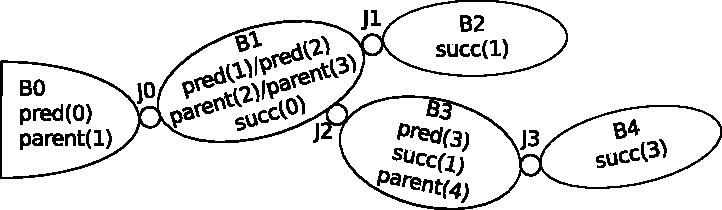
\includegraphics[width=0.7\textwidth]{mbg.pdf}
  \caption{MultiBody graph}
  \label{fig:mbg}
\end{figure}

The geometric relationships between bodies and joints are described through transformations between their bases. Transformations are described in the Spacial Vector Algebra chapter of "Rigid Body Dynamics Algorithm" by Roy Featherstone \cite{featherstone:book:2007}.

Let A and B be Cartesian frames with origins O and P respectively. Let $\mathbf{t}$ be the coordinate vector expressing $\overrightarrow{OP}$ in A. And $\mathbf{R}$ be the rotation matrix that transforms 3D vectors from A to B coordinates.
The transformation from A to B for a motion vector is then defined by:
\begin{equation}
  ^BX_A =
  \begin{pmatrix}
    \mathbf{R} & \mathbf{0} \\
    -\mathbf{R}\hat{\mathbf{t}} & \mathbf{R} \\
  \end{pmatrix}
\end{equation}
Its inverse is:
\begin{equation}
  {^BX_A}^{-1} = ^AX_B =
  \begin{pmatrix}
    \mathbf{R}^T & \mathbf{0} \\
    \hat{\mathbf{t}}\mathbf{R}^T & \mathbf{R}^T \\
  \end{pmatrix}
\end{equation}
The transformation from A to B for a force vector is defined by:
\begin{equation}
  ^BX_A^* =
  \begin{pmatrix}
    \mathbf{R} & -\mathbf{R}\hat{\mathbf{t}} \\
    \mathbf{0} & \mathbf{R} \\
  \end{pmatrix}
\end{equation}
Its inverse is:
\begin{equation}
  ^BX_A^{-*} = ^AX_B^* =
  \begin{pmatrix}
    \mathbf{R}^T & \hat{\mathbf{t}}\mathbf{R}^T \\
    \mathbf{0} & \mathbf{R}^T \\
  \end{pmatrix}
\end{equation}

Each joint $J_i$ is defined in the referential of its predecessor body by a static transformation $X^x_i = \{\mathbf{R}^x_i, \mathbf{t}^x_i\}$ from the base of the body to the base of the joint.
Each joint $J_i$ is associated with a motion subspace which representation matrix is denoted $\mathbf{S}_i$. Each column of $\mathbf{S}_i$ described a degree of freedom of $J_i$ its upper part for the rotations and lower for translations.
\begin{equation}
  \mathbf{S}_i =
  \begin{pmatrix}
    S^R_{i,0} & \cdots &
    S^R_{i,j} & \cdots &
    S^R_{i,dof} \\
    S^t_{i,0} & \cdots &
    S^t_{i,j} & \cdots &
    S^t_{i,dof}
  \end{pmatrix}
\end{equation}

For a given joint configuration $q$, the transformation due to the joint $J_i$ from its base to the base of its successor body is denoted \\$X^J_i(q) = \{\mathbf{R}^J_i(q), \mathbf{t}^J_i(q)\}$.

The transformation between $B_{\lambda(i)}$ and $B_i$ is denoted $X^{PtS}_i(q) = \{\mathbf{R}^{PtS}_i, \mathbf{t}^{PtS}_i\}$ (PtS stands for "Parent to Son") can then be computed as:
\begin{equation}
  X^{PtS}_i(q) = ^iX_{\lambda(i)}(q) = X^J_i(q) X^x_i
  \label{eq:PtS}
\end{equation}

Let $\kappa(i) =\{0, i_1, i_2 ... i\}$ be the list of indexes of successive bodies going from $B_W$ to $B_i$.
It can easily be computed by adding iteratively the parent of the current body:

\begin{algorithm}
  \caption{Joint Path to $B_i$}
  \label{JP}
\begin{algorithmic}
  \State {$j = i$, $\kappa(i)=[i]$}
  \While {$j \neq 0$}
  \State {$j = \lambda(j)$}
  \State {$\kappa(i) = [\kappa(i),\ j]$}
  \EndWhile
\end{algorithmic}
\end{algorithm}

The transformation from the World base to $B_i$ is denoted \\ $^iX_W(q) = \{^i\mathbf{R}_W(q), ^i\mathbf{t}_W(q)\}$.
The formula \ref{eq:PtS} can be used iteratively on every body of the robot to obtain the expression of $^iX_W(q)$.

We obtain the full expression of $^iX_W$ as:
\begin{equation}
  ^iX_W(q) = \prod_{j\in\kappa(i)}X^J_j(q) X^x_j = \prod_{j\in\kappa(i)}\ ^jX_{\lambda(j)}
  = ^iX_{\kappa(1)}\ ^{\kappa(1)}X_{\kappa(2)} \dots ^{\kappa(\text{end}-1)}X_{W}
\end{equation}

Which can be computed recurcively by the following algorithm:

\begin{algorithm}
  \caption{Forward Kinematics}
  \label{FK}
\begin{algorithmic}
  \For {$i = 0:n_J$}
  \If {$\lambda(i) \neq -1$} $^iX_W = ^iX_{\lambda(i)}\ ^{\lambda(i)}X_W$
  \Else $\ ^iX_W = X^{PtS}_i$
  \EndIf
  \EndFor
\end{algorithmic}
\end{algorithm}

In the following section, we provide some detailed description of how to compute $X_J(q)$ for a variety of usefull joints.
Using the joint descriptions and the Forward Kinematics algorithm, we are now able to explicit a relationship between the articular parameter of the robot $q$ and the 3D position and orientation of any frame, point, vector, or any geometric quantity defined in the frame of a body of the robot expressed in any other frame.
Given a transformation $^pX_i$ defined in the frame of $B_i$, its value in the world frame is given by $^pX_W(q) = ^pX_i\ ^iX_W(q)$

\subsection{Joints formulations}
\label{sub:joints_formulations}

The entire geometry of our system is described by the list of static transformations $X^x_j$ and of joint transformations $X^J_j(q)$.

Let us considere a joint $J$ that governs the transformation between two frames $F_1=\{O_1, x_1, y_1, z_1\}$ and $F_2=\{O_2, x_2, y_2, z_2\}$.
The most common types of joint encountered in robotics systems is the revolute joint, that allows a rotation around a fixed axis.
If $J$ is a revolute joint arount the axis $(O_1,z_1)$ with parameter $q$, its motion subspace, rotation and translation are as follows:

\begin{tabular}{|c|c|c|c|}
  \hline
  Joint type & $S$ & $Rotation$ & $translation$ \\
  \hline
  Revolute $(O_1,z_1)$
  &
  $\begin{pmatrix}
    0 \\ 0 \\ 1 \\ 0 \\ 0 \\ 0
  \end{pmatrix}$
  &
  $\begin{pmatrix}
    1 & 0 & 0 \\
    0 & \cos(q) & \sin(q) \\
    0 & -\sin(q) & \cos(q) \\
  \end{pmatrix}$
  &
  $\bf{0}_{3\times1}$
  \\
  \hline
\end{tabular}

Similar formulas can be devised for rotations around any other axis, provided that $R$ describes the rotation of angle $q$ around that axis.

In the case of a prismatic joint, all rotations are blocked, and only one translation along a given axis is allowed.
For a prismatic joint along $x_1$, we have the following formulas:

\begin{tabular}{|c|c|c|c|}
  \hline
  Joint type & $S$ & $Rotation$ & $translation$ \\
  \hline
  Prismatic $(x_1)$
  &
  $\begin{pmatrix}
    0 \\ 0 \\ 0 \\ 1 \\ 0 \\ 0
  \end{pmatrix}$
  &
  $\bf{1}_{3\times3} $
  &
  $\begin{pmatrix}
    q \\ 0 \\ 0
  \end{pmatrix}$
  \\
  \hline
\end{tabular}

Planar joints are also often used in robotics. A planar joint describes a plan sliding on another plan, assuming that the normal to both plans is $z_1 = z_2$ this type of joint allows free rotation of $F_2$ around $z_1$ and translations along $x_1$ and $y_1$. We denote $q = \{q_1, q_2, q_3\}$ the joint parameters, $q_1$ corresponding to the rotation and $q_2,\ q_3$ to the translations. We get:

\begin{tabular}{|c|c|c|c|}
  \hline
  Joint type & $S$ & $Rotation$ & $translation$ \\
  \hline
  Planar $(z_1)$
  &
  $\begin{pmatrix}
    0 & 0 & 0 \\ 0 & 0 & 0 \\ 1 & 0 & 0 \\ 0 & 1 & 0 \\ 0 & 0 & 1 \\ 0 & 0 & 0
  \end{pmatrix}$
  &
  $\begin{pmatrix}
    1 & 0 & 0 \\
    0 & \cos(q_1) & \sin(q_1) \\
    0 & -\sin(q_1) & \cos(q_1) \\
  \end{pmatrix}$
  &
  $\begin{pmatrix}
    \cos(q_1)q_2 - \sin(q_1)q_3 \\ \sin(q_1)q_2 + \cos(q_1)q_3 \\ 0
  \end{pmatrix}$
  \\
  \hline
\end{tabular}

A spherical joint blocks all translations and allows all rotations. This joint mut be parameterized by a 3D rotation. The space of 3D rotations $SO(3)$ can be represented in many different ways.
The simplest and most intuitive way to parameterize $SO(3)$ is to use Euler Angles.
It comes down to decomposing the 3D rotation into a succession of three 1D rotations around different axis.
For example, the roll, pitch, yaw is a succession of a rotation of $F_1$ around its $x$ axis, followed by a rotation of the resulting frame around its $y$ axis and a rotation of the resulting frame around its $z$ axis.
The rotation matrix for such a rotation is given by:
\begin{equation}
  \bf{R} =
  \begin{pmatrix}
    1 & 0 & 0 \\
    0 & \cos(q_3) & \sin(q_3) \\
    0 & -\sin(q_3) & \cos(q_3) \\
  \end{pmatrix}
  +
  \begin{pmatrix}
    \cos(q_2) & 0 & -\sin(q_2) \\
    0 & 1 & 0 \\
    \sin(q_2) & 0 & \cos(q_2) \\
  \end{pmatrix}
  +
  \begin{pmatrix}
    \cos(q_1) & \sin(q_1) & 0 \\
    -\sin(q_1) & \cos(q_1) & 0 \\
    0 & 0 & 1
  \end{pmatrix}
\end{equation}

There are many other possible choices of axes to define the a Euler Angle 3D rotation.
The advantage of such formulation is its simplicity and intuitivity.
But they all suffers from singularities like the Gimbal lock, which happens when two of the three rotation axis become aligned.
In such a configuration, the only rotations possible are around the aligned axis and around another axis.
Thus one degree of freedom is lost.
Those singularities are prohibitive for the use of such a formulation in a posture generation (the optimization algorithm could get stuck in them).

One can prove that there is no smooth mapping between $SO(3)$ and $\mathbb{R}^3$ that is free of singularities.
The most common $SO(3)$ representation in robotics uses the subset of $\mathbb{R}^4$ called the unit quaternion.
A quaternion $q = [q_w, q_x, q_y, q_z]$ is a unit quaternion iff $q_w^2+q_x^2+q_y^2+q_z^2 = 1$.
It represents a rotation of angle $\theta$ around an axis $\bf{u}$ such that:
\begin{align}
  q_w &= \cos(\theta/2) \\
  q_x &= \sin(\theta/2)u_x \\
  q_y &= \sin(\theta/2)u_y \\
  q_z &= \sin(\theta/2)u_z \\
\end{align}
The rotation matrix associated with this rotation formulation is:
\begin{equation}
  \bf{R} = 2 \begin{pmatrix}
    q_w^2 +q_x^2-\frac{1}{2} & q_x q_y + q_w q_z & q_x q_z - q_w q_y \\
    q_x q_y - q_w q_z & q_w^2 +q_y^2-\frac{1}{2} & q_y q_z + q_w q_x \\
    q_x q_z + q_w q_y & q_y q_z - q_w q_x & q_w^2 +q_z^2-\frac{1}{2} \\
  \end{pmatrix}
\end{equation}

That formulation does not suffer from singularity, but it requires to maintain 4 parameters for a 3D rotation. And those 4 parameters must satisfy the unit norm constraint.
Given a parameter set $q = \{ q_w, q_x, q_y, q_z\}$ we get the following table.

\begin{tabular}{|c|c|c|c|}
  \hline
  Joint type & $S$ & $Rotation$ & $translation$ \\
  \hline
  Spherical
  &
  $\begin{pmatrix}
    1 & 0 & 0 \\ 0 & 1 & 0 \\ 0 & 0 & 1 \\ 0 & 0 & 0 \\ 0 & 0 & 0 \\ 0 & 0 & 0
  \end{pmatrix}$
  &
  $2 \begin{pmatrix}
    q_w^2 +q_x^2-\frac{1}{2} & q_x q_y + q_w q_z & q_x q_z - q_w q_y \\
    q_x q_y - q_w q_z & q_w^2 +q_y^2-\frac{1}{2} & q_y q_z + q_w q_x \\
    q_x q_z + q_w q_y & q_y q_z - q_w q_x & q_w^2 +q_z^2-\frac{1}{2} \\
  \end{pmatrix}$
  &
  $\begin{pmatrix}
    0 \\ 0 \\ 0
  \end{pmatrix}$
  \\
  \hline
\end{tabular}

Finally, a free joint allows free motion of its successor body with respect to its predecessor body.
It can be viewed as a combination of a spherical joint and 3 perpendicular prismatic joints.
Given a parameter set $q = \{ q_w, q_x, q_y, q_z, t_x, t_y, t_z\}$ we get the following table.

\begin{tabular}{|c|c|c|c|}
  \hline
  Joint type & $S$ & $Rotation$ & $translation$ \\
  \hline
  Spherical
  &
  $\bf{1}_{6\times 6}$
  &
  $2 \begin{pmatrix}
    q_w^2 +q_x^2-\frac{1}{2} & q_x q_y + q_w q_z & q_x q_z - q_w q_y \\
    q_x q_y - q_w q_z & q_w^2 +q_y^2-\frac{1}{2} & q_y q_z + q_w q_x \\
    q_x q_z + q_w q_y & q_y q_z - q_w q_x & q_w^2 +q_z^2-\frac{1}{2} \\
  \end{pmatrix}$
  &
  $\bf{R}^{-1}\begin{pmatrix}
    t_x \\ t_y \\ t_z
  \end{pmatrix}$
  \\
  \hline
\end{tabular}

\subsection{Jacobian computation}
\label{sub:jacobian_computation}

For the sake of solving our problem with a non-linear optimization algorithm, it is necessary to compute the derivatives of every function used as constraint or cost with respect to any variable of the problem.
The transformations $^iX_W$ are used in many functions, therefore, having an efficient algorithm to compute their derivatives and the derivatives of any transformation defined in $B_i$ is necessary.

\subsection{Formulation of external forces, stability equation and Torque computation}
\label{sub:formulation_of_external_forces_stability_equation_and_torque_computation}

\subsubsection{External Forces}
\label{subsub:external_forces}

For a robot to interact with the real world, its geometric description is not enough.
The robot will be subject to forces applied on its bodies by the exterior world, those can be generated by contacts with the environment or with another actor (human, other robot, manipulated object...), by the effect of physical forces like gravitation or magnetism, or by contacts between two bodies of the robot.
Our posture generator must take those "External forces" into account, be able to estimate the stability of the robot and the internal torques generated in the joints.

An external force applied on a rigid body is called a wrench and is composed of a force part and a moment part(sometimes called couple).
Let $w$ be a wrench, $w|_F^O$ is the expression of $w$ applied on the point $O$ in the frame $F$.
We denote $f|_F$ the expression of the force of $w$ in $F$ and $m|_F^O$ the expression of its moment part in $F$ calculated at the point $O$.

\begin{equation}
  w|_F^O = \left\{ \begin{array}{r}
    m|_F^O\\
    f|_F\\
  \end{array} \right\}
\end{equation}

Note that the expression of the moment part on a different point $P$ follows the following formula:

\begin{equation}
  m|_F^P = m|_F^O + \overrightarrow{PO} \wedge f|_F
\end{equation}

From here we drop the subscript $F$ for clarity.

\subsubsection{Static stability}
\label{subsub:static_stability}

We denote $g$ the acceleration of gravitaty on earth $g = 9.81 m.s^{-2}$.
The wrench associated with action of the gravity of a body of mass $M$ which center of mass is denoted $G$ with $\vec{z}$ the upward vertical vector in the world frame is:
\begin{equation}
  w_g|^G = \left\{ \begin{array}{r}
     0 \\
     -Mg\vec{z} \\
  \end{array}\right\}
\end{equation}

A solid is statically stable if it satisfy the Euler-Newton Equation. We considere a rigid body on which $m$ external forces $w_i$ are applied. We denote $P$ the application point on which the equation is calculated:
\begin{equation}
  \sum\limits_i w_i|^P + w_g|^P = 0
\end{equation}
Which is equivalent to:
\begin{equation}
\left\{
\begin{array}{r}
  \sum\limits_i m_i|^P + \overrightarrow{GP}\wedge Mg\vec{z} = 0 \\
  \sum\limits_i f_i - Mg\vec{z} = 0 \\
\end{array}
\right.
\end{equation}

This equation can be simplified by applying it on the center of mass of the body as:
\begin{equation}
\left\{
\begin{array}{r}
  \sum\limits_i m_i|^G = 0 \\
  \sum\limits_i f_i - Mg\vec{z} = 0 \\
\end{array}
\right.
\label{eq:stability}
\end{equation}

Satisfying \ref{eq:stability} ensures the stability of a rigid body.
In some cases, an articulated robot is considered as a rigid body and this equation can be used to ensure its stability.
It is only valid if the robot can generate infinite torques in its articulations, or at least if we are sure that the robot is able to generate large enough torques.

\subsubsection{Center of mass projection}
\label{subsub:center_of_mass_projection}

In the case where all the wrenches applied to the body are due to unilateral punctual contacts with points that all lay on the same horizontal plan, the stability criterion \ref{eq:stability} can be simplified.We denote $P_i$ the application point of wrench $w_i$ and $O$ is the origin of the horizontal plane.
The wrench generated by a unilateral punctual contact is a pure force, its moment part is null on the contact point.

\begin{equation}
\left\{
\begin{array}{r}
  \sum\limits_i \overrightarrow{OP_i}\wedge f_i - \overrightarrow{OG} \wedge Mg\vec{z} = 0 \\
  \sum\limits_i f_i - Mg\vec{z} = 0 \\
\end{array}
\right.
\end{equation}

We can write $\overrightarrow{OG} = \overrightarrow{OG_p} + z_G\vec{z}$ with $G_P$ the projection of $G$ on the horizontal plan. Replacing in the moment equation gives:

\begin{equation}
  \sum\limits_i \overrightarrow{OP_i}\wedge f_i - \sum\limits_i\overrightarrow{OG_P} \wedge f_i = 0
\end{equation}

The forces $f_i$ also can be separated into their normal and tangential parts: $f_i = f_i^n\vec{z} + f_i^t$, $G$ and $P_i$ can be written as $\overrightarrow{OG_P} = G_x \vec{x} + G_y\vec{y}$ and $\overrightarrow{OP_i} = P_{ix} \vec{x} + P_{iy} \vec{y}$. We get:

\begin{align}
  \sum\limits_i \overrightarrow{OP_i}\wedge f_i^n\vec{z} = \sum\limits_i\overrightarrow{OG_P} \wedge f_i^n\vec{z} \\
\sum\limits_i \left\{\begin{array}{r} P_{iy}f_i^n\\-P_{ix}f_i^n\end{array}\right\}
= \left\{\begin{array}{r} G_{y}\\-G_{x}\end{array}\right\} \sum\limits_if_i^n\\
  \overrightarrow{OG_P} = \frac{\sum\limits_i \overrightarrow{OP_i} f_i^n}{\sum\limits_if_i^n}
\end{align}

Since all the contacts are unilateral and with the same plan, all the $f_i^n$ are positive.
For any set of $f_i^n\geq0$, $G_P$ is a barycentre with positive coefficients of the set of all $P_i$.
Any point $G_P$ that is included in the convex hull of all the $P_i$ is a solution.

Thus we have the property: A rigid body that has all its contacts with the environment being punctual, unilateral and all laying on the same horizontal plan $P$ is stable if and only if the projection of its center of mass on $P$ is inside the convex hull of all its contact points.

\subsubsection{Torque limits}
\label{subsub:torque_limits}

In general, satisfying equation \ref{eq:stability} is not enough to ensure that a robot can be statically stable.
The joint torques that are required to hold the posture must be within the physical capabilities of the robot, namely, its torque limits.
We denote $\tau_i^-$ and $\tau_i^+$ the minimal and maximal torques that can be generated by the robot's actuators on joint $J_i$.
Note that in some cases, the torque limits are not constant and can depend on the joint articular parameters $\tau_i^-(q)$ and $\tau_i^+(q)$.
For example it is the case with the Atlas robot that is hydraulically actuated.

Featherstone \cite{featherstone:book:2007} proposes a reccursive algorithm to compute the torques, accelerations and velocites generated in a multi articulated system by a set of external forces called the Inverse Dynamics Algorithm.
For the purpose of generating statically stable postures, the velocities and accelerations are useless.
Thus, we simplify the algorithm to fit our needs that we call the Inverse Static Algorithm.

The algorithm first computes the generalized forces $f^G_i$ applied on each body, it is the sum of the action of gravity and of the external forces applied on a body at the origin of the world frame, expressed in the world frame.
Then, the generalized forces are used to compute the torques.

\begin{algorithm}
  \caption{Inverse Static Algorithm}
  \label{IS}
\begin{algorithmic}
  \For {$i = 0:n_B$}
  \State $f^G_i = \mathbf{I}^W \mathbf{X}^W_i \mathbf{a}^G - {\mathbf{X}^W_i}^*f_i^{ext}$
  \EndFor
  \For {$i = n_J-1:0$}
  \State $\tau_i = {f^G_i}^T S_i$
  \If {$pred(i) \neq -1$}
  \State $f^G_{pred(i)} += {\mathbf{X}^{PtS}_i(q)}^{-*} f^G_i$
  \EndIf
  \EndFor
\end{algorithmic}
\end{algorithm}

We can write the torques as a function of the joint parameters and the external forces $\tau(q,f)$.
The torque limit constraint writes as:
\begin{equation}
  \tau^- \leq \tau(q,f) \leq \tau^+
\end{equation}

\subsection{Torque derivation}

\begin{algorithm}
  \caption{Inverse Static Matrix form}
  \label{ISmatrix}
\begin{algorithmic}
  \For {$i = 0:n_B$}\\
  $f^G_i =
  \begin{pmatrix}
    \mathbf{m}^{G}_i \\ \mathbf{f}^{G}_i
  \end{pmatrix}
  =
  \mathbf{I}^W
  \begin{pmatrix}
    {\mathbf{R}^W_i} & \mathbf{0} \\
    -{\mathbf{R}^W_i}\widehat{\mathbf{t}^W_i} & {\mathbf{R}^W_i} \\
  \end{pmatrix}
  \begin{pmatrix}
    \mathbf{ac} \\ \mathbf{af}
  \end{pmatrix}
  -
  \begin{pmatrix}
    {\mathbf{R}^W_i} & -{\mathbf{R}^W_i}\widehat{\mathbf{t}^W_i} \\
    \mathbf{0} & {\mathbf{R}^W_i} \\
  \end{pmatrix}
  \begin{pmatrix}
    \mathbf{m}^{ext}_i \\ \mathbf{f}^{ext}_i
  \end{pmatrix}
  $
  \EndFor
  \For {$i = n_J-1:0$}
  \State $\tau_i = {f^G_i}^T S_i$
  \If {$pred(i) \neq -1$}
  \State $f^G_{pred(i)} =
  \begin{pmatrix}
    \mathbf{m}^{G}_{pred(i)} \\ \mathbf{f}^{G}_{pred(i)}
  \end{pmatrix}
  +=
  \begin{pmatrix}
    {\mathbf{R}^{PtS}_i}^T & \widehat{\mathbf{t}^{PtS}_i}{\mathbf{R}^{PtS}_i}^T \\
    \mathbf{0} & {\mathbf{R}^{PtS}_i}^T \\
  \end{pmatrix}
  \begin{pmatrix}
    \mathbf{m}^{G}_i \\ \mathbf{f}^{G}_i
  \end{pmatrix}
  $
  \EndIf
  \EndFor
\end{algorithmic}
\end{algorithm}

The computation of the torque jacobian $\frac{\partial \tau}{\partial q}$ with respect to the articular parameters is done by differenciating the previous algorithm.

Note the following relations:
\begin{align}
  \frac{\partial \mathbf{R}_i^W \mathbf{u}}{\partial q_j}
  &= \mathbf{R}_i^W \mathbf{u} \wedge \omega_{i,j}
  = \mathbf{R}_i^W \widehat{\mathbf{u}} \omega_{i,j}
  \\
  \frac{\partial \mathbf{R}_i^W \mathbf{t}^W_i\wedge \mathbf{u}}{\partial q_j}
  &= \mathbf{R}_i^W \mathbf{v}_{i,j} \wedge \mathbf{u}
  + \mathbf{R}_i^W \left(\mathbf{t}^W_i\wedge\mathbf{u}\right) \wedge \omega_{i,j}\\
  &= -\mathbf{R}_i^W \widehat{\mathbf{u}} \mathbf{v}_{i,j}
  + \mathbf{R}_i^W \widehat{\left(\widehat{\mathbf{t}^W_i}\mathbf{u}\right)} \omega_{i,j}
\end{align}

Let's differentiate the first equation of \ref{ISmatrix} w.r.t $q_j$.

\begin{align}
  A &=
  \begin{pmatrix}
    {\mathbf{R}^W_i} & \mathbf{0} \\
    -{\mathbf{R}^W_i}\widehat{\mathbf{t}^W_i} & {\mathbf{R}^W_i} \\
  \end{pmatrix}
  \begin{pmatrix}
    \mathbf{ac} \\ \mathbf{af}
  \end{pmatrix} \\
  B &=
  \begin{pmatrix}
    {\mathbf{R}^W_i} & -{\mathbf{R}^W_i}\widehat{\mathbf{t}^W_i} \\
    \mathbf{0} & {\mathbf{R}^W_i} \\
  \end{pmatrix}
  \begin{pmatrix}
    \mathbf{m}^{ext}_i \\ \mathbf{f}^{ext}_i
  \end{pmatrix} \\
  f^G_i &= \mathbf{I}^WA-B\\
  \frac{\partial A}{\partial q_j} &=
  \begin{pmatrix}
    \mathbf{R}^W_i \widehat{\bf ac} \omega_{i,j}\\
    -{\mathbf{R}^W_i}\widehat{\left(\widehat{\mathbf{t}^W_i}\bf ac \right)}\omega_{i,j}
    + {\mathbf{R}^W_i}\widehat{\bf ac} v_{i,j} + \mathbf{R}^W_i \widehat{\bf af} \omega_{i,j}\\
  \end{pmatrix}
  \\
  \frac{\partial B}{\partial q_j} &=
  \begin{pmatrix}
    - {\mathbf{R}^W_i}\widehat{\left(\widehat{\mathbf{t}^W_i}\bf \mathbf{f}^{ext}_i \right)}\omega_{i,j}
    + {\mathbf{R}^W_i}\widehat{\bf \mathbf{f}^{ext}_i} v_{i,j} + \mathbf{R}^W_i \widehat{\bf \mathbf{m}^{ext}_i} \omega_{i,j}\\
    \mathbf{R}^W_i \widehat{\bf \mathbf{f}^{ext}_i} \omega_{i,j}\\
  \end{pmatrix}
  \\&+
  \begin{pmatrix}
    {\mathbf{R}^W_i} & -{\mathbf{R}^W_i}\widehat{\mathbf{t}^W_i} \\
    \mathbf{0} & {\mathbf{R}^W_i} \\
  \end{pmatrix}
  \begin{pmatrix}
    \frac{\partial \mathbf{m}^{ext}_i}{\partial q} \\ \frac{\partial \mathbf{f}^{ext}_i}{\partial q}
  \end{pmatrix}
\end{align}

Putting all the pieces of $\omega$ and $v$ allows to group all the j-derivatives to obtain the jacobian of $f^G_i$ with a single equation.

\begin{align}
  \bf M &=
  \begin{pmatrix}
    \mathbf{R}^W_i \widehat{\bf ac}  & 0\\
    -{\mathbf{R}^W_i}\widehat{\left(\widehat{\mathbf{t}^W_i}\bf ac \right)}
    + \mathbf{R}^W_i \widehat{\bf af}  & {\mathbf{R}^W_i}\widehat{\bf ac} \\
  \end{pmatrix}
  \\
  \bf N &=
  \begin{pmatrix}
    - {\mathbf{R}^W_i}\widehat{\left(\widehat{\mathbf{t}^W_i}\bf \mathbf{f}^{ext}_i \right)} + \mathbf{R}^W_i \widehat{\bf \mathbf{m}^{ext}_i} & {\mathbf{R}^W_i}\widehat{\bf \mathbf{f}^{ext}_i} \\
    \mathbf{R}^W_i \widehat{\bf \mathbf{f}^{ext}_i} & 0\\
  \end{pmatrix}
  \\
  \frac{\partial f^G_i}{\partial q} &= (\mathbf{I}^W \mathbf{M} - \mathbf{N})\mathbf{Jac}^W_i
  +
  \begin{pmatrix}
    {\mathbf{R}^W_i} & -{\mathbf{R}^W_i}\widehat{\mathbf{t}^W_i} \\
    \mathbf{0} & {\mathbf{R}^W_i} \\
  \end{pmatrix}
  \begin{pmatrix}
    \frac{\partial \mathbf{m}^{ext}_i}{\partial q} \\ \frac{\partial \mathbf{f}^{ext}_i}{\partial q}
  \end{pmatrix}
\end{align}

The derivation of the second equation is obvious:

\begin{align}
  \tau_i &= {f^G_i}^T S_i \\
  \frac{\partial \tau_i}{\partial q} &= S_i^T \frac{\partial f^G_i}{\partial q} \\
\end{align}

Note the following relations:
\begin{align}
  \frac{\partial {\mathbf{R}_i^J}^T \mathbf{u}}{\partial q_j}
  &= - S^R_{i,j} \wedge ({\mathbf{R}_i^J}^T \mathbf{u})
  = \widehat{({\mathbf{R}_i^J}^T \mathbf{u})} S^R_{i,j}
  \\
  \frac{\partial\mathbf{t}^J_i\wedge {\mathbf{R}_i^J}^T  \mathbf{u}}{\partial q_j}
  &= S^t_{i,j} \wedge \left({\mathbf{R}_i^J}^T \mathbf{u}\right)
  - \mathbf{t}^J_i \wedge \left( S^R_{i,j} \wedge \left({\mathbf{R}_i^J}^T \mathbf{u}\right)\right) \\
  &= -\widehat{({\mathbf{R}_i^J}^T \mathbf{u})} S^t_{i,j}
  + \left(\left({\mathbf{R}_i^J}^T \mathbf{u}\right) . {\mathbf{t}^J_i}^T
  - \left( ({\mathbf{R}_i^J}^T \mathbf{u})^T . \mathbf{t}^J_i\right) \mathbf{I}_3\right)S_{i,j}^R\\
\end{align}

The last equation's derivation goes like follows:

\begin{align}
  f^G_{pred(i)} & +=
  \begin{pmatrix}
    {\mathbf{R}^{PtS}_i}^T & \widehat{\mathbf{t}^{PtS}_i}{\mathbf{R}^{PtS}_i}^T \\
    \mathbf{0} & {\mathbf{R}^{PtS}_i}^T \\
  \end{pmatrix}
  \begin{pmatrix}
    \mathbf{m}^{G}_i \\ \mathbf{f}^{G}_i
  \end{pmatrix}
  \\
  & += \begin{pmatrix}
    {\mathbf{R}^{x}_i}^T & \widehat{\mathbf{t}^{x}_i}{\mathbf{R}^{x}_i}^T \\
    \mathbf{0} & {\mathbf{R}^{x}_i}^T \\
  \end{pmatrix}
  \begin{pmatrix}
    {\mathbf{R}^{J}_i}^T & \widehat{\mathbf{t}^{J}_i}{\mathbf{R}^{J}_i}^T \\
    \mathbf{0} & {\mathbf{R}^{J}_i}^T \\
  \end{pmatrix}
  \begin{pmatrix}
    \mathbf{m}^{G}_i \\ \mathbf{f}^{G}_i
  \end{pmatrix}
  \\
  K_i &=
  \begin{pmatrix}
    \widehat{({\mathbf{R}_i^J}^T \mathbf{m}^{G}_i)}
    + \left({\mathbf{R}_i^J}^T \mathbf{f}^{G}_i\right) . {\mathbf{t}^J_i}^T
    - \left( ({\mathbf{R}_i^J}^T \mathbf{f}^{G}_i)^T . \mathbf{t}^J_i\right) \mathbf{I}_3
    & -\widehat{({\mathbf{R}_i^J}^T \mathbf{f}^{G}_i)} \\
    \widehat{({\mathbf{R}_i^J}^T \mathbf{f}^{G}_i)} & 0
  \end{pmatrix}
  \\
  \frac{\partial f^G_{pred(i)}}{\partial q} & -=
  \begin{pmatrix}
    {\mathbf{R}^{x}_i}^T & \widehat{\mathbf{t}^{x}_i}{\mathbf{R}^{x}_i}^T \\
    \mathbf{0} & {\mathbf{R}^{x}_i}^T \\
  \end{pmatrix}
  K_i S_i
\end{align}


The entire algorithm for calculating the torque jacobian w.r.t the articular parameters comes down to:

\begin{algorithm}
  \caption{Torque Jacobian Calculation}
  \label{TJC}
\begin{algorithmic}
  \For {$i = 0:n_B$}
  \State Compute the Jacobian of generalized forces
  \State
  $f^G_i =
  \mathbf{I}^W
  \begin{pmatrix}
    {\mathbf{R}^W_i} & \mathbf{0} \\
    -{\mathbf{R}^W_i}\widehat{\mathbf{t}^W_i} & {\mathbf{R}^W_i} \\
  \end{pmatrix}
  \begin{pmatrix}
    \mathbf{ac} \\ \mathbf{af}
  \end{pmatrix}
  -
  \begin{pmatrix}
    {\mathbf{R}^W_i} & -{\mathbf{R}^W_i}\widehat{\mathbf{t}^W_i} \\
    \mathbf{0} & {\mathbf{R}^W_i} \\
  \end{pmatrix}
  \begin{pmatrix}
    \mathbf{m}^{ext}_i \\ \mathbf{f}^{ext}_i
  \end{pmatrix}
  $
  \State $\bf M =
    \begin{pmatrix}
    \mathbf{R}^W_i \widehat{\bf ac}  & 0\\
    -{\mathbf{R}^W_i}\widehat{\left(\widehat{\mathbf{t}^W_i}\bf ac \right)}
    + \mathbf{R}^W_i \widehat{\bf af}  & {\mathbf{R}^W_i}\widehat{\bf ac} \\
    \end{pmatrix}
    $
  \State
  $\bf N =
  \begin{pmatrix}
    - {\mathbf{R}^W_i}\widehat{\left(\widehat{\mathbf{t}^W_i}\bf \mathbf{f}^{ext}_i \right)}
    + \mathbf{R}^W_i \widehat{\bf \mathbf{m}^{ext}_i}
    & {\mathbf{R}^W_i}\widehat{\bf \mathbf{f}^{ext}_i} \\
    \mathbf{R}^W_i \widehat{\bf \mathbf{f}^{ext}_i} & 0\\
  \end{pmatrix}
  $
  \State $
  \frac{\partial f^G_i}{\partial q} = (\mathbf{I}^W \mathbf{M} - \mathbf{N})\mathbf{Jac}^W_i
  +
  \begin{pmatrix}
    {\mathbf{R}^W_i} & -{\mathbf{R}^W_i}\widehat{\mathbf{t}^W_i} \\
    \mathbf{0} & {\mathbf{R}^W_i} \\
  \end{pmatrix}
  \begin{pmatrix}
    \frac{\partial \mathbf{m}^{ext}_i}{\partial q} \\ \frac{\partial \mathbf{f}^{ext}_i}{\partial q}
  \end{pmatrix}
  $
  \EndFor
  \For {$i = n_J-1:0$}
  \State Compute the Jacobian of torques w.r.t q
  \State $\frac{\partial \tau_i}{\partial q} = S_i^T \frac{\partial f^G_i}{\partial q}$
  \If {$pred(i) \neq -1$}
  \State $\mathbf{K} =
  \begin{pmatrix}
    \widehat{({\mathbf{R}_i^J}^T \mathbf{m}^{G}_i)}
    + \left({\mathbf{R}_i^J}^T \mathbf{f}^{G}_i\right) . {\mathbf{t}^J_i}^T
    - \left( ({\mathbf{R}_i^J}^T \mathbf{f}^{G}_i)^T . \mathbf{t}^J_i\right) \mathbf{I}_3
    & -\widehat{({\mathbf{R}_i^J}^T \mathbf{f}^{G}_i)} \\
    \widehat{({\mathbf{R}_i^J}^T \mathbf{f}^{G}_i)} & 0
  \end{pmatrix}$
  \State $f^G_{pred(i)} += {\mathbf{X}^{PtS}_i(q)}^{-*} f^G_i$
  \State $\frac{\partial f^G_{pred(i)}}{\partial q} -=
  \begin{pmatrix}
    {\mathbf{R}^{x}_i}^T & \widehat{\mathbf{t}^{x}_i}{\mathbf{R}^{x}_i}^T \\
    \mathbf{0} & {\mathbf{R}^{x}_i}^T \\
  \end{pmatrix}
  \mathbf{K} S_i$
  \EndIf
  \EndFor
\end{algorithmic}
\end{algorithm}


\section{Use all those quantities to write an optimization problem}
\label{sec:use_all_those_quantities_to_write_an_optimization_problem}

Variable q,f,tau

Cost function

How to write constraints:
Bounds
Linear part
NonLinear part

\subsection{Formulation of joint limits}
\label{sub:formulation_of_joint_limits}

\subsection{Formulation of collisions}
\label{sub:formulation_of_collisions}

\subsection{Stability}
\label{sub:stability}

\subsection{Torque limits}
\label{sub:torque_limits}

\subsection{Force in friction cone}
\label{sub:force_in_friction_cone}

\section{Contact with the environment}
\label{sec:contact_with_the_environment}

\subsection{Frame contact}
\label{sub:frame_contact}

\subsection{stability constact vs geometry contact}
\label{sub:stability_constact_vs_geometry_contact}

\section{Contact inclusion/Non inclusive contacts}
\label{sec:contact_inclusion_non_inclusive_contacts}















%%%%%%%%%%%%%%%%%%%%%%%%%
%  SECTION FORMULATION  %
%%%%%%%%%%%%%%%%%%%%%%%%%

\section{Formulation}

Here we present the basic formulation of a PG problem.

The free-flyer, the articular space and the forces being the usual variables.

Presentation of all the constraints and their formulation
\begin{itemize}
  \item Joint limits
  \item Auto-collision
  \item Collisions with environment
  \item Contacts with environment
  \item Stability
  \item Torque limits
\end{itemize}

